\chapter{Lecture 17: Exponential and gamma distributions}
So far we have only learned about one continuous distribution, the uniform distribution. \\

\noindent One of the last discrete distributions that we learned about was the Poisson distribution (section \ref{lambda poisson}). \\

\noindent Let $X$ be a discrete random variable with $X \sim$ Poi($\lambda$). Then $X$ counts how many occurrences happen, on average, within one interval of some continuum (like time or length). Suppose that we know, for sure, that exactly one occurrence, call it occurrence $A$, has happened in one interval, call it interval $I$ (i.e., we are supposing that we know $X = 1$). \\

\noindent We didn't go into too much detail about the Poisson distribution, but it is a built in feature of this distribution that the exact \textit{location} of occurrence $A$, within interval $I$, is random, and is uniformly distributed. In other words, if we know that occurrence $A$ happened in interval $I$, then the Poisson distribution assumes that it could have happened anywhere in interval $I$ with \textit{equal probability}. \\

\noindent The \textbf{Poisson process} (not covered in this course) is a mathematical object that is used to model events that follow a Poisson distribution in time. The Poisson process is one of the most important random processes in probability theory; useful for modelling radioactive decay of atoms, the times when customers arrive at a place of business, the number of mutations in a sequence of DNA, and rainfall, among many other examples. The poisson distribution, the \textit{exponential distribution}, and the \textit{gamma distribution}, all can be derived from the Poisson process. We will meet the latter two distributions in this lecture.

\section{Exponential distribution} \label{exponential distribution}
We will soon see that the pdf, $f(x)$, of an exponential distribution, is always decreasing, and that the mode is at $x = 0$. \\

\noindent When occurrences follow a Poisson distribution in time, the intervals between the occurrences, i.e., the waiting times from one occurrence to the next, follow an exponential distribution. We will now show that this is true, and thus derive the exponential distribution from the Poisson distribution. \\

\noindent Suppose that $X \sim$ Poi($\lambda$), and suppose that the continuum is time (measured in units of 1 second). Let $T$ denote the waiting time until the \textit{first} occurrence (i.e., the amount of time from when we start measuring until we observe 1 occurrence). \textbf{Then $\boldsymbol{T}$ is a continuous random variable.} \\

\noindent We interpret $P(T > t)$ to be the probability that we have not had any occurrences yet (i.e., that $X = 0$) by time $t$. We will now find the cdf of $T$, then from this we will find the pdf of $T$, which will be the pdf of the exponential distribution. \\

\noindent Recall that $\lambda$ is the average number of occurrences per unit of continuum. The probability that $X = 0$ (i.e., that there has been no occurrences), after 1 second, is given by the pmf of Poi($\lambda$). The probability that $X = 0$, after 2 seconds, is given by the pmf of Poi(2$\lambda$) (since there are twice as many occurrences, on average, in two units of the continuum). It follows that, in general, \textbf{the probability that $\boldsymbol{X = 0}$, after $\boldsymbol{t}$ seconds, is given by the pmf of Poi($\boldsymbol{\lambda t}$)} (since there are $t$ times the number of occurrences, on average, in $t$ units of the continuum). \\

\noindent Recall, by the definition of a cdf, that $F(t) = P(T \leq t)$. In words, $F(t)$ is the probability that we observe the first occurrance before time $t$. Now,
\begin{align*}
F(t) & = P(T \leq t) \\
      & = 1 - P(T > t)  \tag{probability measure axiom 1} \\
       & = 1 - P(X = 0), \;\;\; \text{at time $t$}. \tag{by our definition of $T$}
\end{align*}
As discussed, $P(X = 0)$, at time $t$, is given by the pmf of Poi($\lambda t$). So,
\begin{align*}
F(t) & = 1 - \frac{(\lambda t)^0}{0!}\e^{-\lambda t} \tag{by the pmf of Poi($\lambda t$), section \ref{lambda poisson}} \\
	& = 1 - \e^{-\lambda t}.
\end{align*}
Now that we have the cdf, $F(t)$, we can find the pdf, $f(t)$, by differentiating $F(t)$ (see section \ref{cdf(continuous)}). We have
\begin{align*}
F'(t)  & = \frac{d}{dt}\brac{1 - \e^{-\lambda t}} \\
	& = -\frac{d}{dt}\brac{\e^{-\lambda t}} \tag{since $\frac{d}{dt}(1) = 0$} \\
	& =  \lambda \e^{-\lambda t} \tag{simple chain, see section \ref{simplest chain}}
\end{align*}
Where $t$ is time, so $t \geq 0$. This is the \textbf{pdf of the exponential distribution:} \label{exponential pdf}

  	\bigskip
	
	\hfil\fbox{
	\begin{minipage}{0.4\columnwidth}{
	
	\vskip 0.02cm
	\begin{center}
	$\displaystyle{f(x) = \left\{ \begin{array}{ll}
	\lambda\e^{-\lambda x}, & \; \text{if} \; x \geq 0 \smallskip \\ 
	0, & \; \text{if} \; x < 0
	\end{array} \right. }$
	\end{center}
	}
	\end{minipage}}
	\bigskip
	
\noindent The exponential distribution takes parameter $\lambda$ (which is sometimes referred to as the \textbf{rate} parameter), and is written \textbf{Exponential($\boldsymbol{\lambda}$)} for short. Sometimes, the exponential distribution is expressed in terms of $\beta = \frac{1}{\lambda}$, which is called the \textbf{scale} parameter; take care with books and software to double check which convention is being used. \label{rate (exponential)} \\

\noindent Below are 3 graphs of Exponential($\lambda$), corresponding to different choices of $\lambda$. 
\begin{center}
	\begin{tikzpicture}[scale = 2]
	\draw [very thick, samples=200,smooth, domain = 0.01:3] plot (\x,{1/2*exp(-1/2*\x)});
	\draw [very thick, gray, samples=200,smooth, domain = 0.01:3] plot (\x,{1*exp(-1*\x)});
	\draw [very thick, blue, samples=200,smooth, domain = 0.01:3] plot (\x,{2*exp(-2*\x)});
	\draw [->,gray] (-0.1,0) -- (3.3,0) node [below right] {$x$};
	\draw [->,gray] (0,-0.1) -- (0,2.3) node [above left] {$y$};
	\draw (0,1/2) node [left] {$\lambda = \frac{1}{2}$};
	\draw [gray] (0,1) node [left] {$\lambda = 1$};
	\draw [blue] (0,2) node [left] {$\lambda = 2$};
	\foreach \x in {1,2,3}{
	\draw (\x,0) node {\tiny$|$} node [below = 1mm] {$\x$};
	}
	\end{tikzpicture}
\end{center}

\subsection{Cdf of exponential distribution} \label{exponential cdf 1}
During section \ref{exponential distribution}, we found that the cdf, $F(x)$, of Exponential($\lambda$) is

  	\bigskip
	
	\hfil\fbox{
	\begin{minipage}{0.4\columnwidth}{
	
	\vskip 0.02cm
	\begin{center}
	$\displaystyle{F(x) = \left\{ 
	\begin{array}{ll}
	1 - \e^{-\lambda t}, & \; \text{if} \; x \geq 0 \smallskip \\
	0, & \; \text{if} \; x < 0
	\end{array} \right. }$
	\end{center}
	}
	\end{minipage}}
	\bigskip

\noindent It is possible, alternatively, to derive this result using the fact (from section \ref{cdf(continuous)}) that, for the pdf of any continuous disribution,
\[
F(x) = \int_{-\infty}^x f(t) \; dt.
\]
For Exponential($\lambda$), when $x < 0$ this integral evaluates to $0$ since $f(x) = 0$ when $x < 0$. For $x \geq 0$ the integral becomes
\begin{align*}
F(x)  & = 0 + \int_0^x \lambda \e^{-\lambda t} \; dt \\
	& = \squac{-\frac{\lambda}{\lambda}\e^{-\lambda t}}_0^x \tag{integral formula for } \\
	& = -\e^{-\lambda x} + \e^0 \\
	& = 1 - \e^{-\lambda x}.
\end{align*}

\subsection{Example}
Sketch the cdf of Exponential($\lambda$) and check that it satisfies the three conditions from section \ref{cdf(continuous)}. \\

\solution
\noindent To sketch the cdf of Exponential($\lambda$), we start by recognising that $\e^{-\lambda x}$ is a decreasing (and concave up) curve, like the ones from the graph in section $\ref{exponential distribution}$. Now, $-\e^{-\lambda x}$ (the negative of this), gives an upside down version (i.e., it flips it accross the $x$-axis), giving an increasing (and concave down) curve, like the one in graph $A$ below. Then, $1-\e^{-\lambda x}$ is obtained by adding 1 to the graph everywhere (translating the graph up the $y$-axis by 1), which gives graph $B$ below:  
\begin{center}
\begin{minipage}{0.4\textwidth}
	\begin{center}
	\begin{tikzpicture}
	\draw [gray] (0,1.3) node {Graph $A$};
	\draw [very thick] plot [samples = 200, domain = -0.1:2.6, smooth] (\x,{-exp(-\x)});
	\draw [->,gray] (-0.2,0.1) -- (3,0.1) node [below] {$x$};
	\draw [->,gray] (0,-1.5) -- (0,0.5) node [above left] {$y$};
	\draw (0,-1.04) node [rotate = 90] {$|$} node [below left] {$-1$}; 
	\end{tikzpicture}
	\end{center}
\end{minipage}
\begin{minipage}{0.1\textwidth}
\begin{center}
	\begin{tikzpicture}
	\draw [gray] (0,0) node [rotate = 90] {$\longrightarrow$} node [rotate = 90, above] {Translate up by $1$};
	\end{tikzpicture}
\end{center}
\end{minipage}
\begin{minipage}{0.4\textwidth}
	\begin{center}
	\begin{tikzpicture}
	\draw [gray] (0,2.6) node {Graph $B$};
	\draw [very thick] plot [samples = 200, domain = -0.1:2.6, smooth] (\x,{1-exp(-\x)});
	\draw [->,gray] (-0.2,0) -- (3,0) node [below] {$x$};
	\draw [->,gray] (0,-0.2) -- (0,1.8) node [above left] {$y$};
	\draw (0,1.04) node [rotate = 90] {$|$} node [above left] {$1$}; 
	\end{tikzpicture}
	\end{center}
\end{minipage}
\end{center}
We have sketched $F(x)$ for $x \geq 0$. For $x < 0$ we have $F(x) = 0$, so our final graph of $F(x)$ looks like:
\begin{center}
	\begin{tikzpicture}
	\draw [very thick] (-1,0) -- (0,0);
	\draw [very thick] plot [samples = 200, domain = 0:2.6, smooth] (\x,{1-exp(-\x)});
	\draw [->,gray] (-1,0) -- (3,0) node [below] {$x$};
	\draw [->,gray] (0,-0.2) -- (0,1.8) node [above left] {$y$};
	\draw (0,1.04) node [rotate = 90] {$|$} node [above left] {$1$}; 
	\end{tikzpicture}
\end{center}
Looking at the graph, we can see that $F(x) \rightarrow 0$ as $x \rightarrow -\infty$, and $F(x) \rightarrow 1$ as $F(x) \rightarrow \infty$. Also, the graph is non-decreasing. Hence the three conditions are satisfied. We can double check these limits by considering
\[
\lim_{x \rightarrow \infty} \brac{1-\e^{-\lambda x}} = 1 \qquad \text{and} \qquad F(x) = 0 \; \text{for all $x < 0$, by definition}
\]

\subsection{Example} \label{ex17.1}
What is the probability that $X > a$ for an exponentially distributed random variable? \\

\solution
Let $X \sim$ Exponential($\lambda$). Then
\begin{align*}
P(X > a) & = 1 - P(X \leq a) \tag{probability measure axiom 1} \\
	      & = 1 - \int_{-\infty}^a f(x) \; dx \\
	      & = 1 - \brac{\int_{-\infty}^0 0 \; dx + \int_0^\infty \lambda e^{-\lambda x} \; dx} \tag{definition of pdf of Exponential($\lambda$)} \\
	      & = 1 - \squac{-\e^{-\lambda x}}_0^a \tag{FTC, and an integral formula} \\
	      & = 1 - \brac{-\e^{-\lambda a} - (-\e^0)} \\
	      & = \e^{-\lambda a}.
\end{align*}
Alternatively, we could have used the following integral
\[
P(X > a) = \int_a^\infty f(x) \; dx.
\]
Which would have given the same result.

\subsection{Example}
Magnitudes of earthquakes (on the Richter scale) can be modelled by an exponential distribution with $\lambda = \frac{1}{2.4}$. \\

\noindent Find the probability that the magnitude of an earthquake lies between 2 and 3. Then find the probability that the magnitude exceeds 3. Finally, what is the probability that the magnitude is \textit{equal} to 3? \\

\solution
Let $X$ measure the magnitude of the earthquakes. Then $X \sim$ Exponential($\lambda$). Hence the probability that the magnitude is between 2 and 3 is
\begin{align*}
P(2 < X < 3) & = \int_2^3 f(x) \; dx \\
		& = F(3) - F(2) \tag{by FTC, see section \ref{cdf(continuous)}} \\
		& = (1-\e^{-\frac{1}{2.4}\times3}) - (1-\e^{-\frac{1}{2.4}\times2}) \tag{cdf from section \ref{exponential cdf 1}} \\
		& = \e^{-\frac{2}{2.4}} - \e^{-\frac{3}{2.4}} \\
		& \approx 0.1481.
\end{align*}
The probability that the magnitude exceeds 3 is
\begin{align*}
P(X > 3) & = 1 - P(X \leq 3) \\
	& =1 - (1 - \e^{-\frac{3}{2.4}}) \tag{cdf from section \ref{exponential cdf 1}} \\
	& = \e^{-\frac{3}{2.4}} \\
	& \approx 0.2865.
\end{align*}
The probability that the magnitude is equal to 3 is $P(X = 3) = 0$, see section \ref{subsec15.1} for reason.

\section{The gamma function} \label{gamma function}
\noindent We will soon learn about the gamma distribution, and it will turn out the exponential distribution is a special case of the gamma distribution. \\

\noindent As it turns out, the exponential distribution and the gamma distribution both have probability density functions of the form
\[
f(x) = \boldsymbol{c}\;x^{\boldsymbol{p}} \e^{-\lambda x}, \qquad \text{for $x \geq 0$}.
\]
Where $ \boldsymbol{c}$ and $ \boldsymbol{p}$ are some real valued constants. For Exponential($\lambda$), the constants are $c = \lambda$, and $p = 0$, giving $f(x) = \lambda x^0 \e^{-\lambda x} = \lambda \e^{-\lambda x}$ (as expected). \\

\noindent The gamma distribution inherits its name from its use of an important function called the \textbf{gamma function}. In general, when the constant, $c$, is chosen, it needs to be done in such a way that the resulting $f(x)$ is a viable pdf; this means, in part, that we need to ensure that
\[
\int_{-\infty}^\infty \boldsymbol{c}\;x^{\boldsymbol{p}} \e^{-\lambda x} \; dx = 1.
\]
By linearity, we can pull $c$ out the front of the integral. Also, $f(x)$ is defined to be zero for all $x < 0$. So the equation simplifies to
\[
\boldsymbol{c} \; \int_{0}^\infty x^{\boldsymbol{p}} \e^{-\lambda x} \; dx = 1.
\] 
The gamma function, $\Gamma(\alpha)$, is very closely related to this integral; the difference is that the gamma function sets both $c$ and $\lambda$ equal to 1, and (for slightly obscure reasons) we replace the dummy variable, $p$, by $\alpha - 1$. This gives 

  	\bigskip
	
	\hfil\fbox{
	\begin{minipage}{0.4\columnwidth}{
	
	\vskip 0.02cm
	\begin{center}
	$\displaystyle{\Gamma(\alpha) = \int_{0}^\infty x^{\boldsymbol{\alpha - 1}} \e^{-x} \; dx}$
	\end{center}
	}
	\end{minipage}}
	\bigskip

\noindent For some special values of $\alpha$, this integral can be done exactly. For all other values it is found using numerical approximation techniques. \\

\noindent So, we have just intuitively justified the role that the gamma function plays in the gamma distribution, by implying that it is involved in making sure that the constant, $c$, is viable. We will now look at a different way to understand the gamma function. \\

\noindent The expression $k!$ only makes sense when $k$ is a natural number or zero. For example, we can find $3! = 3\times2\times1$, while $0.25!$ or $(-0.1)!$ do not make any sense. The gamma function is actually a solution to the problem of not having a continuous factorial function; that is, it is an extension of the factorial function to all real numbers (except the non-positive integers, for which the gamma function is undefined). \\

\noindent The pmf of the Poisson distribution (a discrete distribution) uses the constant
\[
\frac{\lambda^k}{k!} \tag{see section \ref{poi(lambda)}}
\]
We will soon see that the pmf of the gamma distribution (a continuous distribution) uses a very similar constant, in which the factorial expression is replaced by a gamma function:
\[
\boldsymbol{c} = \frac{\lambda^\alpha}{\Gamma(\alpha)} \tag{see section \ref{gamma distribution1}}
\]
\subsection{Important properties of the gamma function} \label{gamma properties}
\noindent We will prove some of the following facts in section \ref{sec18.1}, using the definition of the gamma function, after learning a new integration technique.  \\

\noindent As we just mentioned, the gamma function is an extension of the factorial function. Naturally then, we require the gamma function to be equivalent to the factorial function whenever $\alpha$ is a natural number or zero. It turns out that
\[
n! = \Gamma(n + 1), \;\; \text{when $n$ is a natural number or zero}. 
\]   
We can equivalently rewrite this as

  	\bigskip
	
	\hfil\fbox{
	\begin{minipage}{0.42\columnwidth}{
	
	\vskip 0.02cm
	\begin{center}
	$\displaystyle{\Gamma(n) = (n - 1)!},$ $\text{when $n$ is a natural number}$
	\end{center}
	}
	\end{minipage}}
	\bigskip

\noindent Since $0! = 1$ it follows that $\Gamma(1) = (1 - 1)! = 0! = 1$, so

  	\bigskip
	
	\hfil\fbox{
	\begin{minipage}{0.15\columnwidth}{
	
	\vskip 0.02cm
	\begin{center}
	$\displaystyle{\Gamma(1) = 1}$
	\end{center}
	}
	\end{minipage}}
	\bigskip

\noindent Notice that $\Gamma(1)$ (rather than $\Gamma(0)$) is equal to $0!$.  \\

\noindent Now, factorials have the property that,
\[
\alpha! = \alpha\; \underbrace{\boldsymbol{(\alpha-1)(\alpha - 2)\ldots\times2\times1}}_{(\alpha - 1)!} = \alpha\;\boldsymbol{(\alpha-1)!}
\]
The gamma function mimics this property by obeying the following rule, which applies to all $\alpha$ in the domain of the gamma function (not just natural numbers):

  	\bigskip
	
	\hfil\fbox{
	\begin{minipage}{0.3\columnwidth}{
	
	\vskip 0.02cm
	\begin{center}
	$\displaystyle{\Gamma(\alpha) = (\alpha - 1)\Gamma(\alpha - 1)}$
	\end{center}
	}
	\end{minipage}}
	\bigskip

\noindent One more useful result, which we will prove in section \ref{gamma1/2 = sqrt(pi)}, is

  	\bigskip
	
	\hfil\fbox{
	\begin{minipage}{0.2\columnwidth}{
	
	\vskip 0.02cm
	\begin{center}
	$\displaystyle{\Gamma\brac{\frac{1}{2}} = \sqrt{\pi}}$
	\end{center}
	}
	\end{minipage}}
	\bigskip

\noindent We already mentioned briefly that the gamma function is not defined for non-positive integers (i.e., it is defined for all real numbers except negative whole numbers and zero). This means that the graph of the gamma function has asymptotes at each neagtive integer. Below is a graph of $\Gamma(\alpha)$ for $\alpha \in [-4,4]$. The graph has been split into 6 ``pieces'' due to the presence of the asymptotes.

\begin{center}
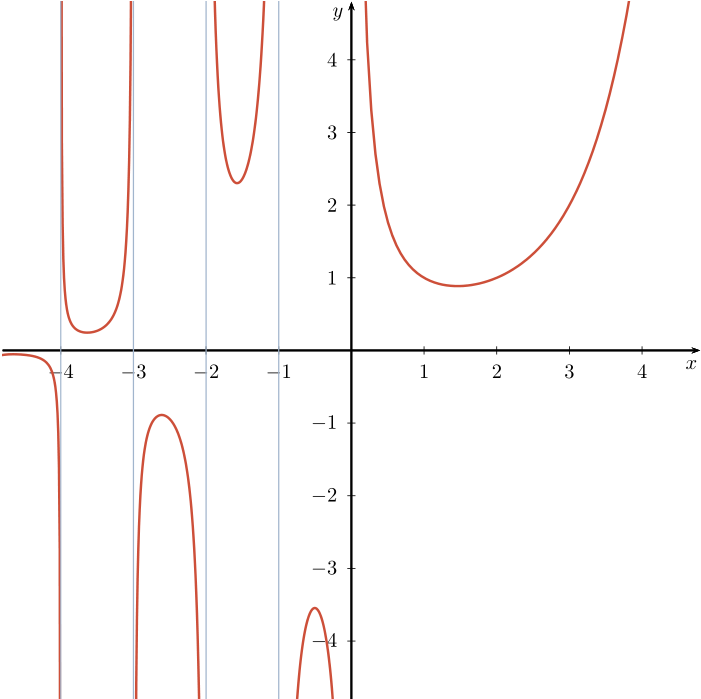
\includegraphics[scale = 0.3]{images/gamma.png}
\end{center}

\section{Gamma distribution} \label{gamma distribution1}
In section \ref{exponential distribution}, we derived the pmf of the exponential distribution by looking at the amount of time leading up to the \textit{first} occurrance in a Poisson distribution. We now do something similar for the gamma distribution. \\

\noindent Let $X \sim$ Poi($\lambda$), where $\lambda$ measures the number of occurrences per 1 second of time. Now define a new random variable, $T$, so that $T$ measures the amount of time leading up to the $k^\text{th}$ occurrence (as opposed to just the first occurrence). Then $T$ is a continuous random variable. \\

\noindent So, we would interpret $P(T > t)$ to be the probability that we have not had $k$ occurrences yet (i.e., that $X < k$) by time $t$. As before, $P(X < k)$, at time $t$, is given by the pmf of Poi($\lambda t$) (see the reasoning behind this in section \ref{exponential distribution}). Furthermore, since $X$ is discrete, we have $P(X < k) = P(X \leq k - 1)$, as $X$ takes no outputs between $k-1$ and $k$. \\

\noindent Let $X \sim $ Poi($\lambda t$). The domain of $X$ is $\set{0,1,2,3,\ldots}$; so,
\begin{align*}
P(X \leq k - 1) & = P(X = 0) + P(X = 1) + \ldots + P(X = k-1) \\
	& = \sum_{\alpha=0}^{k-1}P(X = \alpha) \\
	& = \sum_{\alpha=0}^{k-1}\frac{(\lambda t)^\alpha}{\alpha!}\e^{-\lambda t}. \;\;\;\;\;\;\;\;\; (\dagger) \tag{using the pmf of Poi($\lambda t$), section \ref{lambda poisson}}
\end{align*}

\noindent We now find the cdf, $F(t)$, of $T$, then use this to find the pdf of $T$. We have
\begin{align*}
F(t)   & = P(T \leq t) \tag{definition of a cdf} \\
	& = 1 - P(T > t) \tag{probability measure axiom 1} \\
	& = 1 - P(X < k), \; \text{at time $t$} \tag{by our definition of $T$}  \\
	& = 1 - P(X \leq k-1), \; \text{at time $t$} \tag{since $X$ is discrete} \\
	& = 1 - \sum_{\alpha=0}^{k-1} \frac{(\lambda t)^\alpha}{\alpha!} \e^{-\lambda t } \tag{by ($\dagger$)}
\end{align*}
This is the cdf of the gamma distribution, for $t \geq 0$ (though it is not in a very neat form). To find the pdf, $f(t)$, we differentiate this with respect to $t$. Doing so is not difficult (it involves the product rule and the use of linearity), but there are many steps to simplifying the result, so we will omit the process here (it would be a nice challenging task for the interested reader). The result (after much simplification) is that
\begin{align*}
f(t)  & = \frac{\lambda^\alpha}{(\alpha-1)!}t^{\alpha-1}\e^{-\lambda t} \\
       & = \frac{\lambda^\alpha}{\Gamma(\alpha)}t^{\alpha-1}\e^{-\lambda t} \tag{since $\alpha$ is an integer, so $\Gamma(\alpha) = (\alpha-1)!$}
\end{align*}
Where $t \geq 0$. Replacing the dummy variable, $t$, with $x$, we have the \textbf{pdf of the gamma distribution:} \label{gamma(alpha,lambda)}

  	\bigskip
	
	\hfil\fbox{
	\begin{minipage}{0.65\columnwidth}{
	
	\vskip 0.02cm
	\begin{center}
	$\displaystyle{f(x) = \left\{ \begin{array}{ll}
	\displaystyle{\frac{\lambda^\alpha}{\Gamma(\alpha)}x^{\alpha-1}\e^{-\lambda x}}, & \; \text{if} \; x \geq 0 \smallskip \\ 
	0, & \; \text{if} \; x < 0
	\end{array} \right. }$
	where $\alpha, \lambda > 0$
	\end{center}
	}
	\end{minipage}}
	\bigskip

\noindent The gamma dsitribution takes parameters $\alpha$ and $\lambda$; $\alpha$ is called the \textbf{shape} parameter, and $\lambda$ is called the \textbf{rate}, and some books or software use paremeter $\beta = \frac{1}{\lambda}$, which is called the \textbf{scale} (just as was the case with $\lambda$ in the exponential distribution); hence $\lambda$ is sometimes referred to as the \textbf{inverse scale} parameter. We write \textbf{Gamma($\boldsymbol{\alpha,\lambda}$)} for short. \label{inverse scale gamma} \label{shape gamma} \label{rate gamma} \\

\noindent It is important to emphasize that for a random variable $X \sim $ Gamma($\alpha,\lambda$), the integral
\[
P(a < X < b) = \int_a^b \frac{\lambda^\alpha}{\Gamma(\alpha)}x^{\alpha - 1}\e^{-\lambda x} \; dx 
\]
\textbf{cannot be done exactly}, most of the time. The solutions are generally approximated or looked up using mathematical or statistical software. \\

\noindent Below are some graphs of the gamma distribution for various choices of parameters.
\begin{center}
\begin{tikzpicture}[yscale = 7]
%draw axes
\draw [gray,->] (-0.2,0) -- (7,0) node [below right] {$x$};
\draw [gray,->] (0,-0.2/7) -- (0,1) node [above left] {$f(x)$};
\foreach \y in {0.1,0.2,0.3,0.4,0.5,0.6,0.7,0.8,0.9}{
\draw (0.1,\y) -- (-0.1,\y) node [left] {$\y$}; 
}
\foreach \x in {1,2,3,4,5}{
\draw (\x,0.1/7) -- (\x,-0.1/7) node [below] {$\x$};
}
\draw (4,0.8) node {$\boldsymbol{\lambda = 1}$};
%draw pdfs
\def\alphav{1};
\def\lambdav{1};
\tikzset{declare function={gamma(\z)=(\z-1)!;}}
\def\coefficientv{exp(\alphav*ln(\lambdav))/gamma(\alphav)};
\tikzset{declare function={termone(\x)=exp((\alphav-1)*ln(\x));}}
\tikzset{declare function={termtwo(\x)=exp(-\lambdav*\x);}}
\foreach \t/\colourv in {1/gray,2/red,3/blue,4/black}{
\pgfmathsetmacro\k{\t*20}
\pgfmathsetmacro\l{7/\t}
\pgfmathsetmacro\p{\l-7.5}
\def\alphav{\t};
\draw [very thick,color=\colourv, samples=200,smooth,domain = 0.01:5.5] plot (\x,{\coefficientv*termone(\x)*termtwo(\x)}) node [right = 8mm, below = \p mm] {$\boldsymbol{\alpha = \alphav}$};
}
\end{tikzpicture}
\end{center}
\begin{center}
\begin{tikzpicture}[yscale = 7]
%draw axes
\draw [gray,->] (-0.2,0) -- (7,0) node [below right] {$x$};
\draw [gray,->] (0,-0.2/7) -- (0,1.15) node [above left] {$f(x)$};
\foreach \y in {0.1,0.2,0.3,0.4,0.5,0.6,0.7,0.8,0.9,1,1.1}{
\draw (0.1,\y) -- (-0.1,\y) node [left] {$\y$}; 
}
\foreach \x in {1,2,3,4,5}{
\draw (\x,0.1/7) -- (\x,-0.1/7) node [below] {$\x$};
}
\draw (4,0.8) node {$\boldsymbol{\alpha = 2}$};
%draw pdfs
\def\alphav{2};
\def\lambdav{1};
\tikzset{declare function={gamma(\z)=(\z-1)!;}}
\def\coefficientv{exp(\alphav*ln(\lambdav))/gamma(\alphav)};
\tikzset{declare function={termone(\x)=exp((\alphav-1)*ln(\x));}}
\tikzset{declare function={termtwo(\x)=exp(-\lambdav*\x);}}
\foreach \t/\colourv in {{1/2}/gray,1/red,2/blue,3/black}{
	\pgfmathsetmacro\k{\t*20}
	\pgfmathsetmacro\l{7/\t}
	\pgfmathsetmacro\p{\l-7.5}
	\def\lambdav{\t};
	\draw [very thick,color=\colourv, samples=200,smooth,domain = 0.01:5.5] plot (\x,{\coefficientv*termone(\x)*termtwo(\x)});
}
%labels
\draw (6.3,-0.1/2) node [black] {$\boldsymbol{\lambda = 3}$};
\draw (6.3,0) node [blue] {$\boldsymbol{\lambda = 2}$};
\draw (6.3,0.1/2) node [red] {$\boldsymbol{\lambda = 1}$};
\draw (6.5,0.2/2) node [gray] {$\boldsymbol{\lambda = 1/2}$};
\end{tikzpicture}
\end{center}

\noindent Recall that we derived the pmf of the exponential distribution by looking at the amount of time leading up to the \textit{first} occurrance, i.e. $k = 1$. Since $\alpha$ was our replacement for $k$, we can conclude that Exponential($\lambda$) is a special case of Gamma($\alpha, \lambda$); it is the case with $\alpha = 1$. Indeed, letting $\alpha = 1$ in the pmf of the Gamma distribution gives
\[
f(x) = \frac{\lambda^1}{\Gamma(1)}x^{1-1}\e^{-\lambda x} = \lambda \e^{-\lambda x}.
\]
Which is the pdf of Exponential($\lambda$). \\

\noindent In section \ref{gamma axiom 1}, we will check that the pdf of Gamma($\alpha,\lambda$) satisfies probability measure axiom 1. Then in section \ref{rate/scale gamma}, we will take a deeper look at why $\lambda$ is called the inverse scale parameter.

\section{Memoryless property} \label{memoryless property}
Suppose my friend wants to catch a bus in Japan. When she arrives at the bus stop, the expected wait time is 20 minutes. After 10 minutes, she checks the expected wait time again. Of course, the expected wait time is now 10 minutes. This is an example of a situation where the relevant distribution (of expected waiting times) is not memoryless. \\

\noindent My other friend (I have two) is waiting for a train replacement bus in Melbourne: To begin with, the expected wait time is 20 minutes; 10 minutes later, the expected wait time is 20 minutes; 10 minutes after that, the expected wait time is 20 minutes. This is an example of a situation where the relevant distribution is memoryless. \\

\noindent Only two distributions have the memoryless property: The \textbf{geometric distribution} (discrete) and the \textbf{exponential distribution} (continuous). \\

\noindent Formally, a probability measure has the memoryless property when

  	\bigskip
	
	\hfil\fbox{
	\begin{minipage}{0.45\columnwidth}{
	
	\vskip 0.02cm
	\begin{center}
	$\displaystyle{P(X > a + b \mid X > a) = P(X > b)}$
	\end{center}
	}
	\end{minipage}}
	\bigskip


\subsubsection{Geometric distribution}
\textbf{Proof} \\
Let $X \sim$ Geom($p$). Then,
\begin{align*}
P(X > k) & = 1 - P(X \leq k)  \\
	& = 1 - F(k) \tag{by definition, $F(k) = P(X \leq k)$} \\
	& = 1 - (1-(1-p)^k) \tag{since $F(k) = 1-(1-p)^k$, see section \ref{finite geometric series})} \\
	& = (1-p)^k. \tag{$\bigstar$}
\end{align*}
Now, let $a,b$ be natural numbers. Then
\begin{align*}
P(X > a+b \mid X > a) & = \frac{P(X > a+b \; \textit{and} \; X > a)}{P(X > a)} \tag{dftn of conditional probability} \\
	& = \frac{P(X > a+b)}{P(X > a)} \tag{as $\set{X > a+b} \cap \set{X > a} = \set{X > a+b}$} \\
	& = \frac{(1-p)^{a+b}}{(1-p)^a} \tag{by ($\bigstar$) above} \\
	& = (1-p)^b \tag{index laws} \\
	& = P(X > b).
\end{align*}
Hence $P(X > a+b \mid X > a) = P(X > b)$, which is the definition of the memoryless property, as required. \\

\noindent A famous example (using the geometric distribution) is that of the ``gambler's fallacy.'' Suppose that we are playing roulette, and we are sticking to bets on ``black'' (the probability of landing ``black'' is roughly 47\%). Let $X$ count the number of trials until a win, then $X \sim$ Geom($p$).\\

\noindent Suppose that we bet 7 times in a row, and fail each time. A problem gambler might decide that the odds are now in favour of ``black,'' since the probability of not getting black, so many times in a row, must be very low. The gambler is assuming that
\[
P(X \geq 8 \mid X > 7) \;\;\; \text{is greater than} \;\;\; P(X \geq 1).
\]
But we know, by the memoryless property, that $P(X \geq 7+1 \mid X > 7) = P(X \geq 1)$, which falsifies the gambler's assumption.

\subsubsection{Exponential distribution}
\textbf{Proof} \\
Let $X \sim$ Exponential($\lambda$) and let $a,b$ be natural numbers. Then
\begin{align*}
P(X > a + b \mid X > a) & = \frac{P(X > a + b \; \textit{and} \; X > a)}{P(X > a)} \\
		& = \frac{P(X > a + b)}{P(X > a)} \tag{same reasoning as previous proof} \\
		& = \frac{\e^{-\lambda (a+b)}}{\e^{-\lambda a}} \tag{by result in example \ref{ex17.1}} \\
		& = \e^{-\lambda b} \tag{index laws} \\
		& = P(X > b). \tag{again, by result in example \ref{ex17.1}}
\end{align*}
So the exponential distribution also has the memoryless property, as required.

